\chapter{Procedura testu}
Rozdział ten omawia wszystkie aspekty związane bezpośrednio z przeprowadzaniem procedury testu.
W jej skład wchodzi: dystrybucja aplikacji RTE na poszczególne komputery pomiarowe,
zestawianie połączeń serwer -- klienci RTE, dystrybucja testów, przeprowadzanie procedury testu
oraz zbieranie wyników pomiarów.

\section{Dystrybucja RTE}
Niniejszy benchmark jest aplikacją typu klient -- serwer. Rolę klientów pełni w niej aplikacja
RTE, która służy bezpośrednio do wykonywania testów. Aplikacja ta jest uruchamiana na wielu komputerach,
w związku z tym powstaje problem jej dystrybucji. Problem ten został rozwiązany poprzez rozszerzenie
funkcjonalności serwera benchmarku, o funkcjonalność serwera ftp, udostępniającego do pobrania aplikację RTE. 
A zatem, na każdym komputerze na, którym planowane jest zainstalowanie RTE, wystarczy użyć 
klienta ftp, połączyć się z serwerem benchmarku, a następnie pobrać i rozpakować aplikację.

\section{Tworzenie infrastruktury klient -- serwer}\label{sect:infra}
Komunikacja klient -- serwer została oparta o protokół RMI oraz wsparcie oferowane
mu przez framework Spring 2.0. Niezbędne jest zatem odblokowanie odpowiednich portów,
by komunikacja była możliwa. Standardowo serwer RMI benchmarku nasłuchuje na porcie 1199,
klienci RTE mają natomiast przydzielane numery portów dynamicznie tzn. pierwszy wolny port
większy od 1024. Uruchomienie klienta RTE jest możliwe tylko i wyłącznie, gdy serwer RMI benchmarku
jest uruchomiony i dostępny. Przed rozpoczęciem właściwej procedury testu należy zatem uruchomić
serwer benchmarku i wymaganą liczbę klientów RTE. 

Uruchomienie klienta RTE sprowadza się do dwóch czynności:
\begin{enumerate}
\item Wyedytowania, znajdującego się w głównym katalogu klienta -- pliku ,,rte-config.xml''.
Plik ten wygląda następująco:
\begin{codeblock}
<?xml version="1.0" encoding="UTF-8"?>
<rte-config>
	<server-rmiserver>rmi://HOST_NAME:1199/JDBMeasureRMIServer</server-rmiserver>
</rte-config>
\end{codeblock}
Należy w nim zamienić ciąg znaków ,,HOST\_NAME'' na nazwę lub adres IP serwera testu.
Istnieje również możliwość zmieniany numeru portu ze standardowego 1199 --  z tej opcji należy jednak korzystać
jedynie w sytuacji, gdy serwer benchmarku korzysta z innego portu niż standardowy.
\item Wykonać z lini poleceń (w katalogu głównym klienta RTE) następującą komendę: 
\begin{Verbatim}
java -jar rte.jar
\end{Verbatim}
Zarówno klient RTE jak i aplikacja serwera wymagają do pracy zainstalowania na
komputerze JVM (\english{Java Virtual Machine }~\cite{JVM1}),
w wersji 1.5 lub wyższej.
\end{enumerate}
Na pojedynczym hoście można uruchomić wiele instancji klienta RTE, ponadto nic nie stoi na przeszkodzie
by klient taki znajdował się na komputerze, na którym uruchomiony jest serwer benchmarku.
Takie rozwiązanie nie jest zalecane w sytuacji, gdy serwer benchmarku generuje zauważalne obciążenie
podczas procedury testu, gdyż przekładało by się ono na wyniki pomiarów z RTE. Jeżeli procedura 
uruchamiania wymaganych klientów RTE przebiegnie pomyślnie, infrastruktura testu jest gotowa do użycia.

Warto jest w tym miejscu przyjrzeć się bliżej infrastrukturze benchmarku (zob. rys.~\ref{rys:infrastructure2b}).
\begin{figure}[h]
\begin{center}
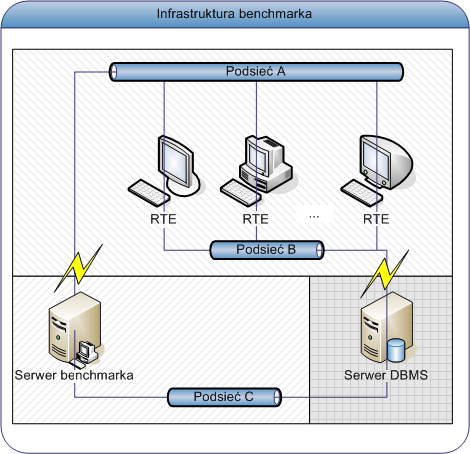
\includegraphics[width=0.8\linewidth]{figures/infrastructure2b.png}
\end{center}
\caption{Infrastruktura benchmarku}\label{rys:infrastructure2b}
\end{figure}
Składa się ona z trzech segmentów/podsieci. Na etapie przygotowywania danych
wykorzystywana jest podsieć C, podsieci A i B nie są wówczas w ogóle potrzebne.
Natomiast podczas procedury testu sytuacja się odwraca -- wówczas to serwer benchmarku
nie komunikuje się bezpośrednio z bazą danych. Warto również zauważyć, iż komunikacja w podsieciach B i~C
odbywa się za pomocą sterowników JDBC, natomiast w sieci A wykorzystywane są protokoły~RMI oraz~ftp.
Podczas inicjalizowania i~finalizowania procedury testu główne obciążenie generowane jest w podsieci~A
ze względu na przesyłanie: klientów RTE, danych testowych i rezultatów testów. W samej zaś procedurze testu
główny ruch przypada na podsieć B. To właśnie ta podsieć, jej parametry techniczne i obciążenie wpływają na 
jakość uzyskiwanych wyników.

\section{Przekazanie skryptów testowych}
Klienci RTE bezpośrednio po połączeniu z serwerem, oczekują na przekazanie skryptów testowych
i zainicjalizowanie procedury testu. W pierwszym kroku serwer przekazuje każdemu RTE
przeznaczonemu do udziału w procedurze testowej -- archiwum ,,test.zip''. Każdy RTE otrzymuje (sekwencyjnie)
inne archiwum ,,test.zip''. RTE po pobraniu archiwum, rozpakowuje je. Następnie ładuje sterownik 
JDBC do bazy danych, testuje połączenie, otwiera strumienie do plików wejściowych i wyjściowych. 
Po pomyślnym wykonaniu powyższych czynności przechodzi w tryb oczekiwania na komendę rozpoczęcia testu.

\section{Wykonywanie testów}
Bezpośrednie wykonywanie testów, rozpoczęcie procedury testu -- następuje po przekazaniu
przez serwer, sygnału synchronizacyjnego -- wszystkim klientom RTE wyznaczonym do udziału w procedurze.
W tym momencie rozpoczyna się zasadnicza procedura testu.

Następnie następuje sekwencja operacji, w której każdy RTE biorący udział w procedurze testowej,
wysyła sygnał synchronizujący do serwera i oczekuje na odesłanie podobnego sygnału synchronizującego. 
Serwer odsyła taki sygnał, gdy otrzyma  sygnały synchronizujące od wszystkich RTE biorących udział w procedurze testowej.
Pomiędzy parami przesłań sygnałów synchronizujących, każdy RTE wykonuje testy, 
zapisując czasy i przechwycone błędy do plików ,,test.time'' oraz ,,test.error''.
Po zakończenia wszystkich testów, każdy RTE wysyła ostatni sygnał synchronizujący. 
Gdy serwer otrzyma ten sygnał od wszystkich RTE ,,wie'', że procedura testu dobiegła końca.
	
Omówione powyżej sygnały synchronizujące są ważnym elementem procedury testu (zob. także punkt~\ref{sub:testscript}). 
To dzięki nim testy składowe zawarte w skryptach wykonywanych na poszczególnych RTE,
są zsynchronizowane -- oznacza to, że niezależnie od różnych czasów zakończenia danego testu,
kolejny test składowy nie rozpocznie się przed zakończeniem, aktualnego testu na wszystkich RTE.

\section{Zbieranie wyników}
Po zakończeniu procedury testu, z każdego RTE biorącego w  niej udział, serwer pobiera poprzez protokół RMI, 
plik ,,testresult.zip''(zob. rys.~\ref{rys:testresultzip}).
\begin{figure}[h]
\begin{center}
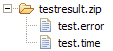
\includegraphics[width=0.3\linewidth]{figures/testresultzip.png}
\end{center}
\caption{Struktura pliku ,,testresult.zip''}\label{rys:testresultzip}
\end{figure}
Plik taki zawiera czasy zarejestrowane podczas procedury, jak i błędy wykonania
operacji na bazie danych. Raz zebrane wyniki mogą być następnie analizowane wielokrotnie
przez serwer benchmarku. Przy czym do analizy takiej, nie jest już wymagane połączenie
z klientami RTE.

\section{Podsumowanie}
Procedura testu składa się zasadniczo z wykonywania przez RTE skryptów testowych,
mierzenia czasów i wymiany sygnałów synchronizujących z serwerem. Wydawałoby się zatem, 
iż nie jest to etap złożony. Należy jednak pamiętać, iż prawidłowość procedury testu
nie sprowadza się jedynie do wykonania wyżej omówionych kroków. Przed rozpoczęciem procedury
testu należy zminimalizować wpływ na wyniki czynników zewnętrznych tj.:
\begin{itemize}
\item Nadmiernego obciążenia sieci i zbyt dużych czasów komunikacyjnych w podsieci B (zob. rys.~\ref{rys:infrastructure2b}).
W procedurze testu należy zatem tak dobrać hosty na, których mają działać aplikacje RTE,
by wpływ tych czynników był jak najmniejszy. Sam benchmark nie niweluje wpływu przepustowości
sieci. Wpływ ten może mieć charakter statyczny -- wynikający z architektury sieci jak i dynamiczny
-- zależny od obciążenia wykorzystywanych segmentów sieci. Nie zaleca się zatem przeprowadzania
testów przez sieć rozległą np.: Internet.
\item Obciążenia przez inne oprogramowanie hostów wykorzystywanych w procedurze testu.
Główną przyczyną jest tutaj dłuższy czas oczekiwania na przydział zasobów tj.: 
dysk twardy, pamięć RAM, karta sieciowa, czas procesora itp.
\item Wykorzystywania DBMS podczas testu przez inne aplikacje.
\end{itemize}
Dopiero uwzględnienie tych czynników w połączeniu z poprawnie wykonaną procedurą testu,
daje w rezultacie istotne dane. 

Korzystając z benchmarku można jednak spróbować oszacować wpływ czynników zewnętrznych 
na wydajność bazy danych widzianą z punktów pomiarowych (hostów RTE). Taki eksperyment
może mieć sens dla konkretnej, istniejącej sieci. W tym celu należy przeprowadzić test dwukrotnie: 
raz w systemie ze zniwelowanym wpływem czynników zewnętrznych, drugi raz w systemie/sieci 
pracującym przy typowym obciążeniu, generowanym przez inne aplikacje. 
Porównując wyniki obu testów można wyciągnąć wnioski,
na które testowane operacje/transakcje zauważalny wpływ mają czynniki zewnętrzne.
Z powyższego eksperymentu może się bowiem okazać, iż ,,wąskim gardłem'' jest 
istniejąca infrastruktura sieci, a nie DBMS, czy testowana baza danych.



